\section{Bias and Variance for learning in 1-D}

Let $f(x) = x^2(1-x)$ where $0 \leq x \leq 1$. We wish to find the `best' linear model (or approximation) for $f$. That is, for functions in the form $g(x; \alpha, \beta) =  \alpha +  \beta x$,  we wish to find the parameters $ \alpha$ and $ \beta$ that minimize the error we would expect to incur if we used the function $g$ to model (or approximate) the function $f$. 
\begin{center}
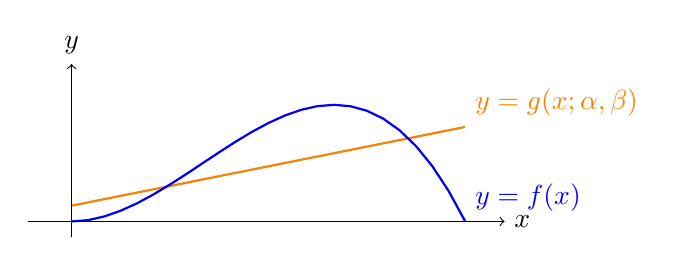
\begin{tikzpicture}[xscale=5,yscale=10]
% \draw[densely dotted] (-.2,-.2) grid (1.2,0.3);
\draw[thick,domain=0:1,variable=\x,orange] plot ({\x},{.02 + .1*\x}) node[above right] {$y = g(x; \alpha, \beta)$};
\draw[thick,domain=0:1,variable=\x,blue] plot ({\x},{\x*\x*(1-\x)}) node[above right] {$y = f(x)$};
  \draw[->] (-.11, 0) -- (1.1, 0) node[right] {$x$};
  \draw[->] (0, -.02) -- (0, .2) node[above] {$y$};
\end{tikzpicture}
\end{center}
For this problem, we will define the error as
\begin{equation*}
\text{Error}(f,g) = \int_0^1 \bigg(f(x) - g(x; \alpha, \beta)\bigg)^2 dx.
\end{equation*} 
Use pencil-and-paper (or Mathematica, WolframAlpha, etc) to find a simplified expression for the error between $f$ and $g$ as a function of the parameters $ \alpha$ and $ \beta$. Find the values of $ \alpha$ and $ \beta$ that minimize this error and the corresponding error.

\noindent\textit{Terminology:} The error we expect to incur when we use our best possible candidate is called the \textit{bias} of the model.

In many practical applications, we only have imperfect knowledge of $f$, and therefore it is impossible to know the parameters of the \textit{best possible} candidate $g(x, \alpha, \beta)$. Often, we must commit to a choice of sub-optimal parameters that are chosen after only a small glimpse of $f$. In this project, we will estimate how much extra error we expect to incur by using an imperfect choice of parameters.


Repeat the following recipe to estimate how well a linear function parameterized by two random data points can be used to approximate $f$.\\
\texttt{Loop until you are confident you have reasonably accurate answers.}
\begin{enumerate}\setlength{\itemsep}{0pt}
    \item \texttt{Generate two random data points on $x_1, x_2 \in [0,1]$.}
    \item \texttt{Using \textbf{only} $x_1$ and $x_2$, compute a `best guess' for parameters $\alpha$ and $\beta$.}
    \item \texttt{Test the performance of your (sub-optimal) parameters by generating new data points and computing the mean square error on the new points. Record the mean square error.}
\end{enumerate}
\texttt{Analyze the mean square error by taking averages and plotting histograms.}

\noindent\textit{Terminology:} When we use `best guess' parameters instead of `best possible' parameters, we can expect to incur error beyond the bias of the model. This `extra error' is called the \textit{variance} of the model.  \\
\vspace*{1cm}	
\noindent For this project, you will need to write the following functions:
\begin{enumerate}
    \item a function that randomly generates two values in $[0,1]$
    \item a function called \texttt{train\_g}.
    \begin{itemize}
        \item Arguments (Input): Two values $x_1$, and $x_2$.
        \item Functionality: Evaluate $y_1:=f(x_1)$ and $y_2:= f(x_2)$. Compute a `best guess' for the parameters $ \alpha$ and $ \beta$ given the points $(x_1,y_1)$ and $(x_2,y_2)$.
        \item Return (Output): $ \alpha$ and $ \beta$.
    \end{itemize}
    \item a function called \texttt{test\_g}.
    \begin{itemize}
        \item Arguments (Input): Parameters $ \alpha$ and $ \beta$.
        \item Functionality: Randomly pick $N$ points in $[0,1]$. For each point, $x_k$, evaluate $f(x_k)$ and $g(x_k;  \alpha,  \beta)$. Compute the average error from the $N$ points as defined by $$E_N = \frac{1}{N}\sum_{k = 1}^N \Big(f(x_k) - g(x_k, \alpha, \beta)\Big)^2$$
        \item Return (Output): $E_N$   
    \end{itemize}
\end{enumerate}

Someone proposes that the variance is so big that it makes the linear model unusable.  They suggest that we should approximate $f$ by a constant function  $h(x;\alpha)$. Repeat the steps above to compute the bias and to the estimate the variance of the constant model. 
